\documentclass{scrartcl}

\usepackage{german}
\usepackage[utf8]{inputenc}  %Umlaute
\usepackage[T1]{fontenc}     %Umlauttrennung
\usepackage{lmodern}         %modernes Schriftbild
\usepackage{amsmath}         %math Umgebungen
\usepackage{graphicx}
\usepackage{hyperref}        %URLs
\usepackage{gensymb}         %Gradzeichen
\usepackage{float}           %Positionierung von Tabellen und Abb
\usepackage{textgreek}


\begin{document}
\begin{titlepage}
  \begin{center}
    \vspace*{1cm}
    \LARGE
    Physikpraktikum für Naturwissenschaftler \\
    \vspace*{1cm}
    \Huge
    \textbf{Versuch: Viskosität} \\
    \vspace*{0.3cm}
    \Large
    Durchgeführt am 17. Januar 2019 \\
    Betreuer: Florian Nägele \\
    \vspace*{2.5cm}
    Gruppe 13 \\
    Felix Burr: felix.burr@uni-ulm.de \\
    Johannes Spindler: johannes.spindler@uni-ulm.de \\
    \vfill 
  \end{center}
  Wir bestätigen hiermit, das Protokoll selbstständig erarbeitet zu haben und in genauer Kenntnis über dessen Inhalt zu sein. \\
  \vspace*{0.8cm}
  \\
  Felix Burr
  \hfill
  Johannes Spindler
\end{titlepage}
\pagebreak
\tableofcontents


\pagebreak

\section{Einleitung}
Unter Viskosität versteht man die innere Reibung die bei realen Fluiden  zwischen benachbarten Fluidschichten auftritt, wenn die Schichten sich aneinander vorbeibewegen. In Flüssigkeiten ist die Viskosität auf Kohäsionskräfte zwischen den Molekülen zurückzuführen, während sie in Gasen durch Stöße zwischen Molekülen verursacht wird. 
Newton definierte die Viskosität mithilfe des folgenden Versuchsaufbaus (siehe Abbildung \ref{fig:Definition}).

\begin{figure}[H]
  \centering
    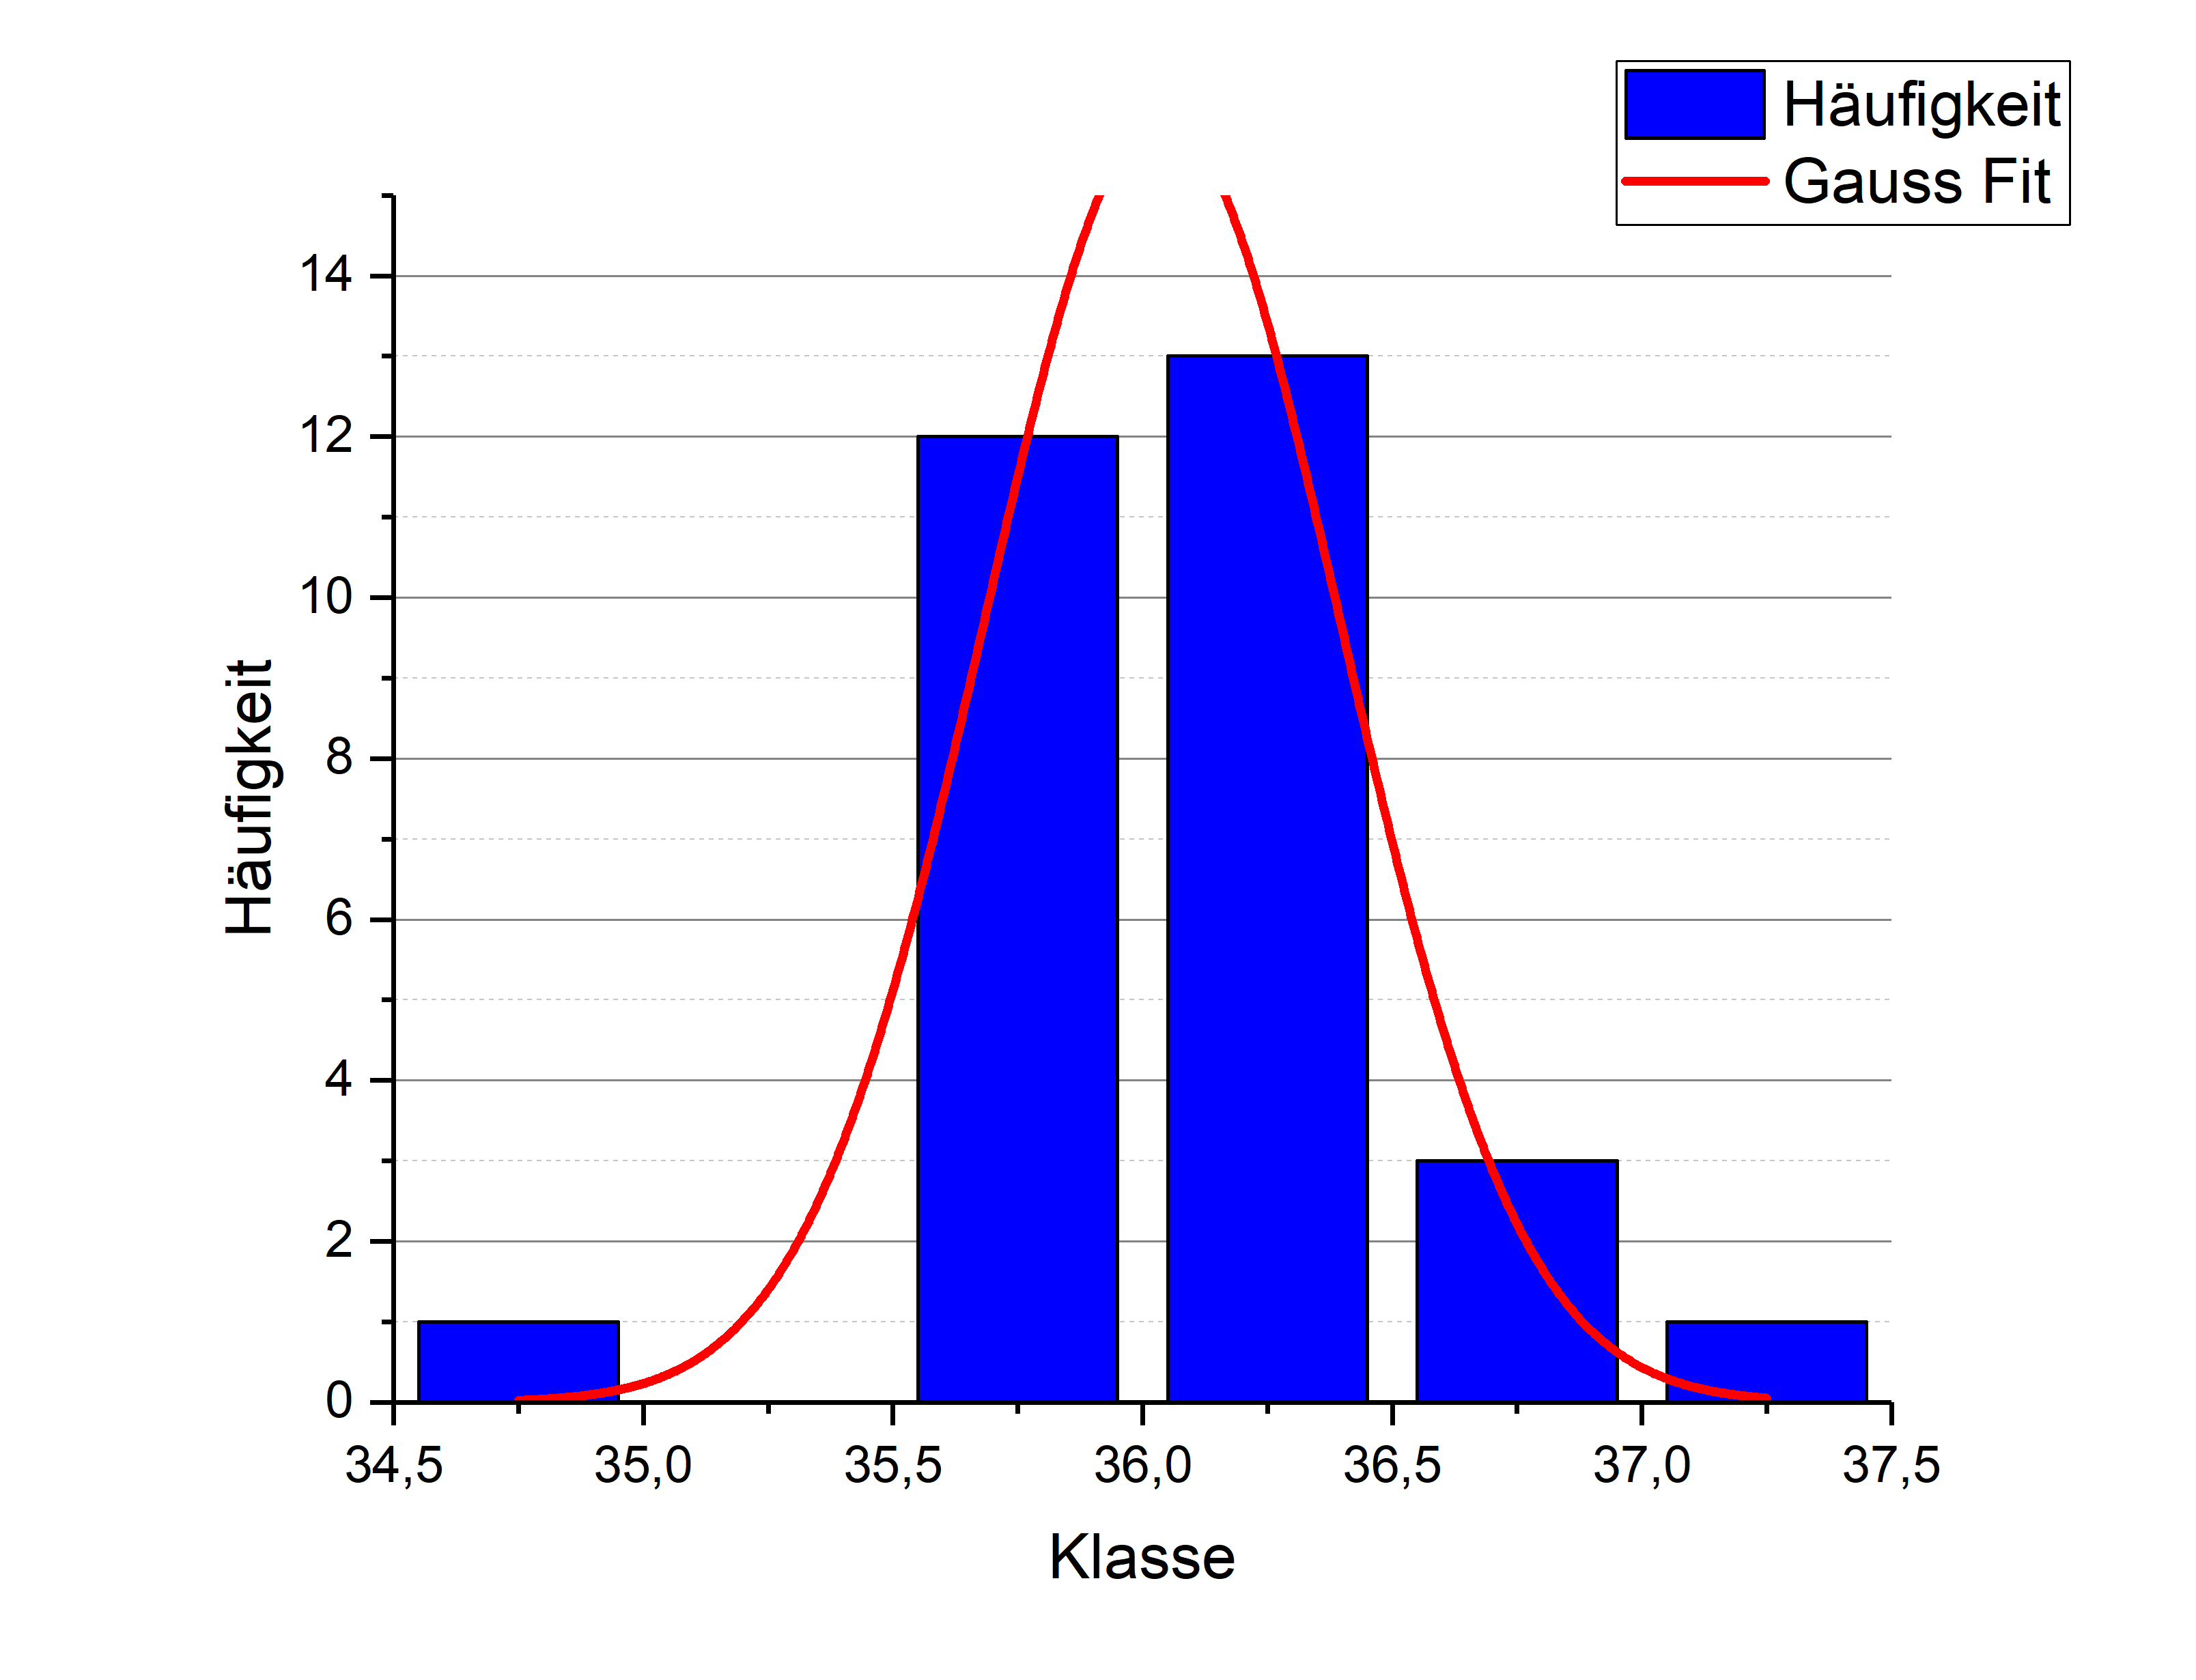
\includegraphics[scale=0.4]{GaussFit.PNG}
  \caption{Aufbau zu Newtons Definition der Viskosität (aus der Versuchsanleitung)}
  \label{fig:Definition}
\end{figure}

Ein zähes Fluid befindet sich zwischen einer beweglichen Platte der Fläche A und einer festen Wand im Abstand $x$. Es greift eine Zugkraft $F$ tangential an der Platte an, sodass die Platte nach einiger Zeit mit konstanter Geschwindigkeit $v$ gleitet. Das heißt, es muss eine entgegengesetzte Reibungskraft $F_{R}$ wirken, die $F$ kompensiert:
\begin{align}
-F_{R} = F = \eta \cdot A \cdot \frac{v}{x}
\end{align}
Hierbei bezeichnet $\eta$ die Viskosität.

Sie soll im ersten Versuch für Getriebeöl mit der Kugelfallmethode und im zweiten Versuch mit dem Kapillarviskosimeter für eine Glycerinlösung unbekannter Konzentration bestimmt werden.




\pagebreak
\section{Bestimmung der Viskosität von Getriebeöl mit der Kugelfallmethode}
\subsection{Versuchsaufbau und Durchführung}
Stahlkugeln in den Größen 1 mm, 2 mm, 3 mm und 4 mm werden nacheinander in ein senkrechtes, mit Getriebeöl gefülltes Rohr geworfen. Für jede Kugelgröße wird davor der durchschnittliche Durchmesser $d$ aus 3 Exemplaren gemessen. Dann wird für 10 Kugeln jeder Größe die Laufzeit $t$ gestoppt, die diese benötigen, um im Rohr um die festgelegte Länge $L$ = 0,30 m hinabzusinken.

Auf die Kugeln wirken die Gewichtskraft $F_{G}$, die Auftriebskraft $F_{A}$ und die Reibungskraft $F_{R}$:
\begin{align}
F_{G} &= \rho_{K} \cdot g \cdot V_{K} \\
F_{A} &= -\rho_{F} \cdot g \cdot V_{K} \\
F_{R} &= -6 \pi \cdot r \cdot \eta \cdot v
\end{align}
Der Index K steht für die Kugel, F steht für das Fluid. Für die Reibungskraft wird hier die Formel für die laminare Umströmung einer Kugel (Radius $r$) nach Stokes verwendet. Es wird angenommen, dass die Geschwindigkeit $v$ auf der Länge $L$ konstant ist, sodass gilt
\begin{align}
F_{G} + F_{A} + F_{R} = 0
\end{align}
Einsetzen und Auflösen nach $\eta$ ergibt
\begin{align}
\eta = \frac{(\rho_{K} - \rho_{F}) \cdot g}{18 \cdot L} \cdot d^2 \cdot t
\label{Viskos}
\end{align}
Dazu werden folgende Literaturwerte verwendet: \\
Dichte Öl: $\rho_{F}$ = 860 kg/m\textsuperscript{3} \\
Dichte Stahl: $\rho_{K}$ = 7800 kg/m\textsuperscript{3} \\
Erdbeschleunigung $g$ = 9,81 m/s\textsuperscript{2}

\subsection{Messwerte und Ergebnisse}
\begin{table}[H]
\captionof{table}{Messwerte für die Kugeldurchmesser d\textsubscript{i}}
\begin{center}
\begin{tabular}{l|l|l|l|l}
Messung   &   d\textsubscript{1} [mm]   &   d\textsubscript{2} [mm]   &   d\textsubscript{3} [mm]   &   d\textsubscript{4} [mm] \\
\hline
1 & 0,99 & 2,00 & 2,99 & 3,99 \\
2 & 1,00 & 1,99 & 2,99 & 3,99 \\
3 & 1,00 & 1,99 & 2,99 & 3,99 \\
\hline
d [mm] & 1,00 & 1,99 & 2,99 & 3,99 \\
\textsigma(d) [mm] & 0,01 & 0,01 & 0,00 & 0,00 
\end{tabular}
\end{center}
\label{tab:Kugeldurchmesser}
\end{table}

\begin{table}[H]
\captionof{table}{Messwerte für die Fallzeiten t\textsubscript{i}}
\begin{center}
\begin{tabular}{l|l|l|l|l}
Messung   &   t\textsubscript{1} [s]   &   t\textsubscript{2} [s]   &   t\textsubscript{3} [s]   &   t\textsubscript{4} [s] \\
\hline
1 & 146 & 36 & 18,31 & 10,21 \\
2 & 143 & 37 & 16,25 & 10,38 \\
3 & 142 & 37 & 17,53 & 10,11 \\
4 & 142 & 37 & 17,00 & 10,56 \\
5 & 144 & 38 & 16,84 &  9,00 \\
6 & 145 & 37 & 17,12 & 10,02 \\
7 & 143 & 38 & 16,81 & 10,06 \\
8 & 144 & 37 & 16,75 &  9,68 \\
9 & 144 & 37 & 16,87 &  9,93 \\
10 & 143 & 37 & 16,81 & 10,75 \\
\hline
t [s] & 143,60 & 37,10 & 17,03 & 10,07 \\
\textsigma(d) [mm] & 1,26 & 0,57 & 0,55 & 0,49 
\end{tabular}
\end{center}
\label{tab:Fallzeiten}
\end{table}

Mit den Mittelwerten $d$, $t$ aus Tabellen \ref{tab:Kugeldurchmesser} und \ref{tab:Fallzeiten} wird in Tabelle \ref{tab:Viskositäten} für jede Kugelgröße die Viskosität berechnet. Um den jeweiligen Größtfehler $\Delta \eta$ zu berechnen werden diese Größtfehler für $d$, $L$, $t$ angenommen: \\
$\Delta d$ = 0,01 mm \\ 
$\Delta L$ = 0,001 m \\
$\Delta t$ = 0,01 s

\begin{table}[H]
\captionof{table}{Berechnete Viskositäten und Größtfehlerberechnungen}
\begin{center}
\begin{tabular}{l|l|l|l|l}
   &   d\textsubscript{1}   &   d\textsubscript{2}   &   d\textsubscript{3}   &   d\textsubscript{4} \\
\hline
\texteta [mPa $cdot$ s] & 1789 & 1859 & 1919 & 2021 \\
2\textDelta d/d & 0,020 & 0,010 & 0,007 & 0,005 \\
\textDelta L/L & 0,003 & 0,003 & 0,003 & 0,003 \\
\textDelta t/t & 0,009 & 0,015 & 0,032 & 0,048 \\
\textDelta \texteta [mPa $cdot$ s] & 58 & 53 & 81 & 115
\end{tabular}
\end{center}
\label{tab:Viskositäten}
\end{table}

Der Mittelwert der Viskosität über die Kugelgrößen ist dann $\eta$ = 1899 mPa $\cdot$ s und dessen Fehler $\Delta \eta$ = 115 mPa $\cdot$ s.
Die gemessene Raumtemperatur betrug 21 \degree C.

\subsection{Statistische Auswertung}
\subsubsection{Bestimmung der Viskosität mittels linearer Regression}
Für die lineare Regression sollen die Wertepaare 1/d\textsuperscript{2}, t für die 4 Kugelgrößen abgebildet werden. Tabelle \ref{tab:linReg} zeigt diese 4 Wertepaare und in Abbildung \ref{fig:linReg} sind sie als Punkte eingetragen.
\begin{table}[H]
\captionof{table}{Wertepaare 1/d\textsuperscript{2}, t für die 4 Kugelgrößen zur linearen Regression}
\begin{center}
\begin{tabular}{l|l|l|l|l}
1/d\textsuperscript{2} [1/mm\textsuperscript{2}] & 1,007 & 0,252 & 0,112 & 0,063 \\
\hline
t [s] & 143,60 & 37,10 & 17,03 & 10,07
\end{tabular}
\end{center}
\label{tab:linReg}
\end{table}

\begin{figure}[H]
  \centering
    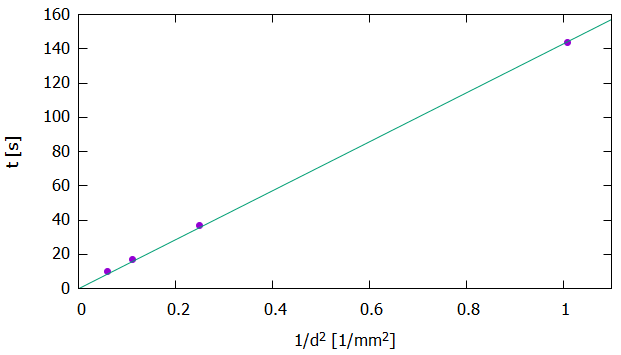
\includegraphics[scale=0.75]{linReg.PNG}
  \caption{Lineare Regression zur Bestimmung der Viskosität}
  \label{fig:linReg}
\end{figure}
Die Steigung $m$ der Regressionsgeraden entspricht dem Term $d^2 \cdot t$ und beträgt $m$ = 142,75 mm\textsuperscript{2}$\cdot$s. Damit ergibt sich mit Gleichung \ref{Viskos} die Viskosität $\eta$ = 1800 mPa$\cdot$s.
\subsubsection{Erstellen eines Histogramms über die Fallzeit}
Zur Erstellung eines Histogramms über die Fallzeit werden nochmals 30 Messungen der Fallzeit mit den 2-mm-Kugeln durchgeführt (siehe Tabelle \ref{tab:Gauss}).
\begin{table}[H]
\captionof{table}{Messung der Fallzeit t zur Erstellung eines Histogramms}
\begin{center}
\begin{tabular}{l|l|l}
t [s]  &  t [s]  &  t [s] \\
\hline
36,31 & 36,04 & 37,43 \\ 
35,39 & 36,37 & 35,93 \\
36,62 & 36,65 & 36,50 \\
36,11 & 36,31 & 35,75 \\
36,25 & 34,81 & 35,87 \\
36,08 & 35,90 & 36,21 \\
35,93 & 35,62 & 36,40 \\
36,40 & 36,31 & 35,79 \\
36,40 & 35,65 & 35,62 \\
35,56 & 36,24 & 36,31 \\
\end{tabular}
\end{center}
\label{tab:Gauss}
\end{table}
Mit dem Plotprogramm Origin werden diese gemessenen Zeiten in sechs Klassen eingeteilt und deren Häufigkeit ermittelt. Außerdem wird eine Normalverteilungskurve an das Histogramm angelegt. Das Ergebnis ist in Abbildung \ref{fig:GaussFit} zu sehen.
\begin{figure}[H]
  \centering
    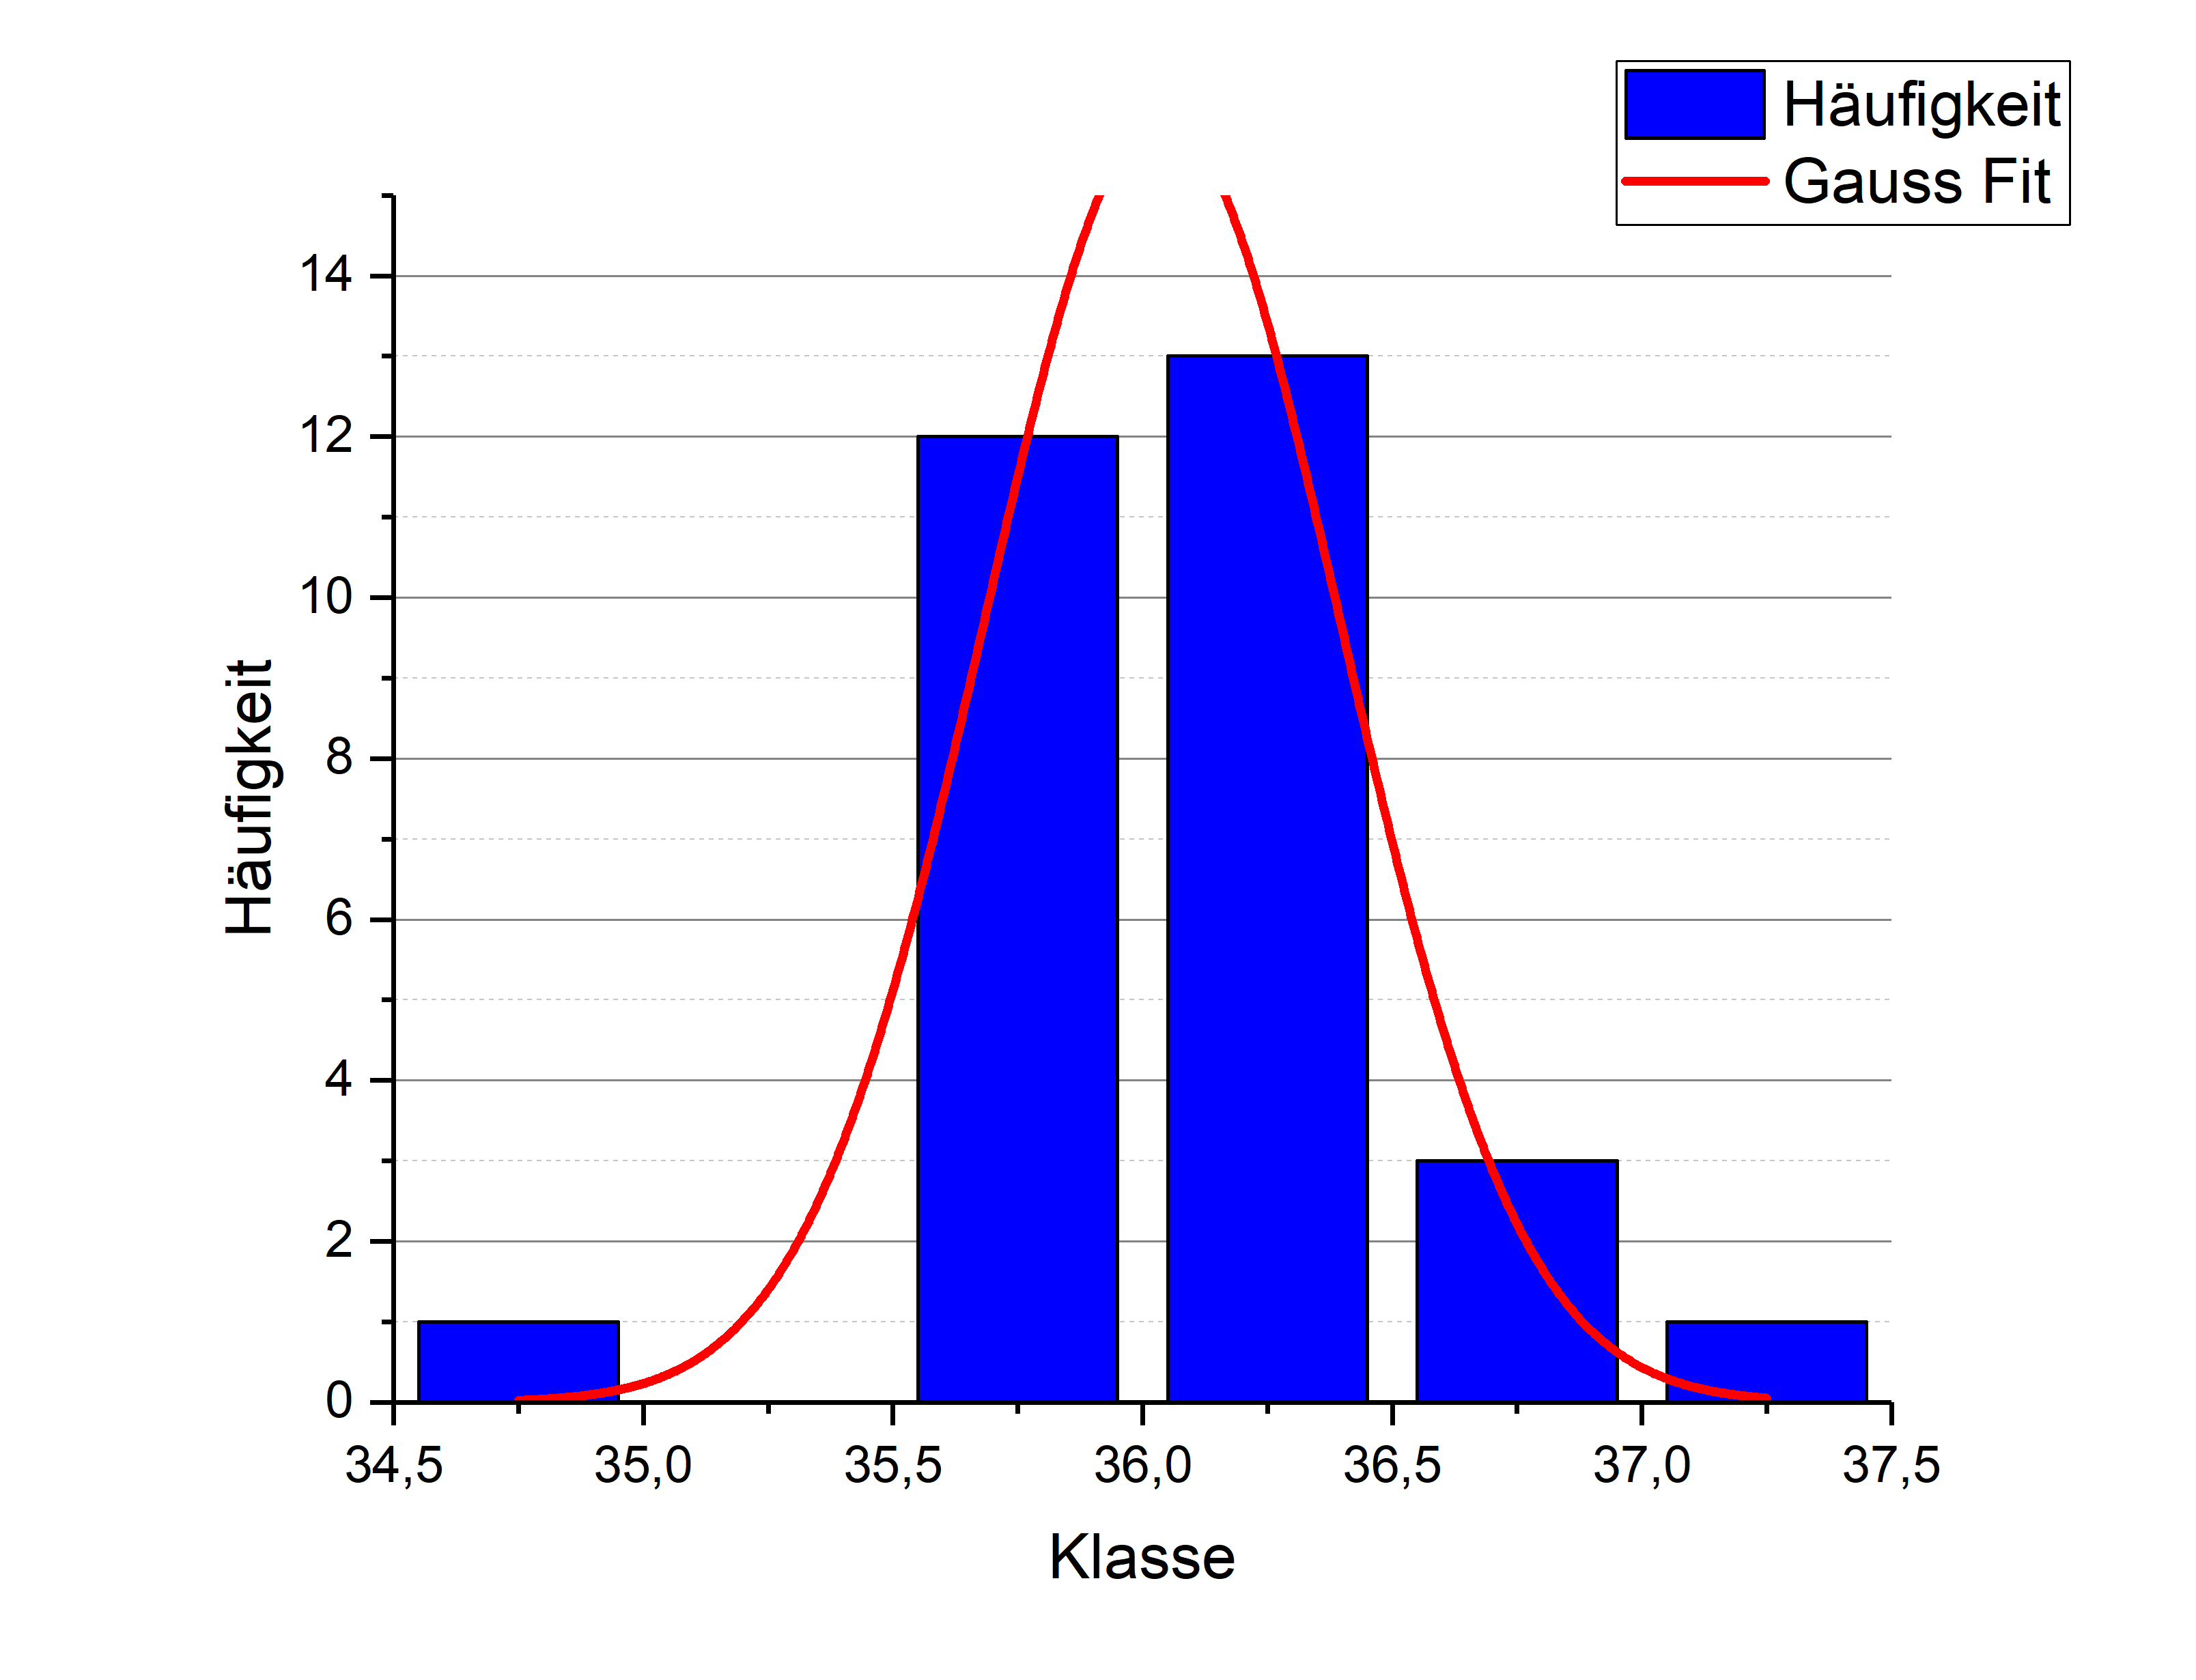
\includegraphics[scale=0.4]{GaussFit.PNG}
  \caption{Histogramm der Fallzeiten der 2-mm-Kugeln und daran angenäherte Normalverteilung)}
  \label{fig:GaussFit}
\end{figure}
Aus dem Histogramm ergibt sich der Mittelwert $t$ = 36,04 s und eine Standardabweichung von \textsigma(t) = 0,36 s.
\subsection{Ergebnisdiskussion}






\pagebreak
\section{Bestimmung der Glycerinkonzentration mit dem Kapillarviskosimeter}
\subsection{Versuchsaufbau und Durchführung}
\subsection{Messwerte und Ergebnisse}
\subsection{Statistische Auswertung}
\subsection{Ergebnisdiskussion}
\end{document}
